\section{Forced System Setup}

\subsection{Time Evolution}



\begin{figure}[htbp]
\centering
\textbf{Electric Field In The Diffusion Problem With Nernst Interaction.}\par\medskip
\begin{subfigure}{.5\linewidth}
\centering
\includegraphics[width=\textwidth]{forced-current-nernstE0.eps}
\caption{}
\label{fig:ef1}
\end{subfigure}%
\begin{subfigure}{.5\linewidth}
\centering
\includegraphics[width =\textwidth]{forced-current-nernstE1.eps}
\caption{}
\label{fig:ef2}
\end{subfigure}\\[1ex]
\begin{subfigure}{\linewidth}
\centering
\includegraphics[width =0.5\textwidth]{forced-current-nernstE2.eps}
\caption{}
\label{fig:ef3}
\end{subfigure}
\caption{Electric field and concentration of $Cu^{+2}$ (green dots) and $SO_4^{-2}$ (blue dots) at (a) $t = 0.448 ns$, (b) $t = 2.24 ns$ and (c) $t = 4.44 ns$}.
\label{fig:test}
\end{figure}

\begin{figure}[htbp]
\centering
\textbf{Electric Potential In The Diffusion Problem With Nernst Interaction.}\par\medskip
\begin{subfigure}{.5\linewidth}
\centering
\includegraphics[width=\textwidth]{forced-current-nernstphi0.eps}
\caption{}
\label{fig:ef1}
\end{subfigure}%
\begin{subfigure}{.5\linewidth}
\centering
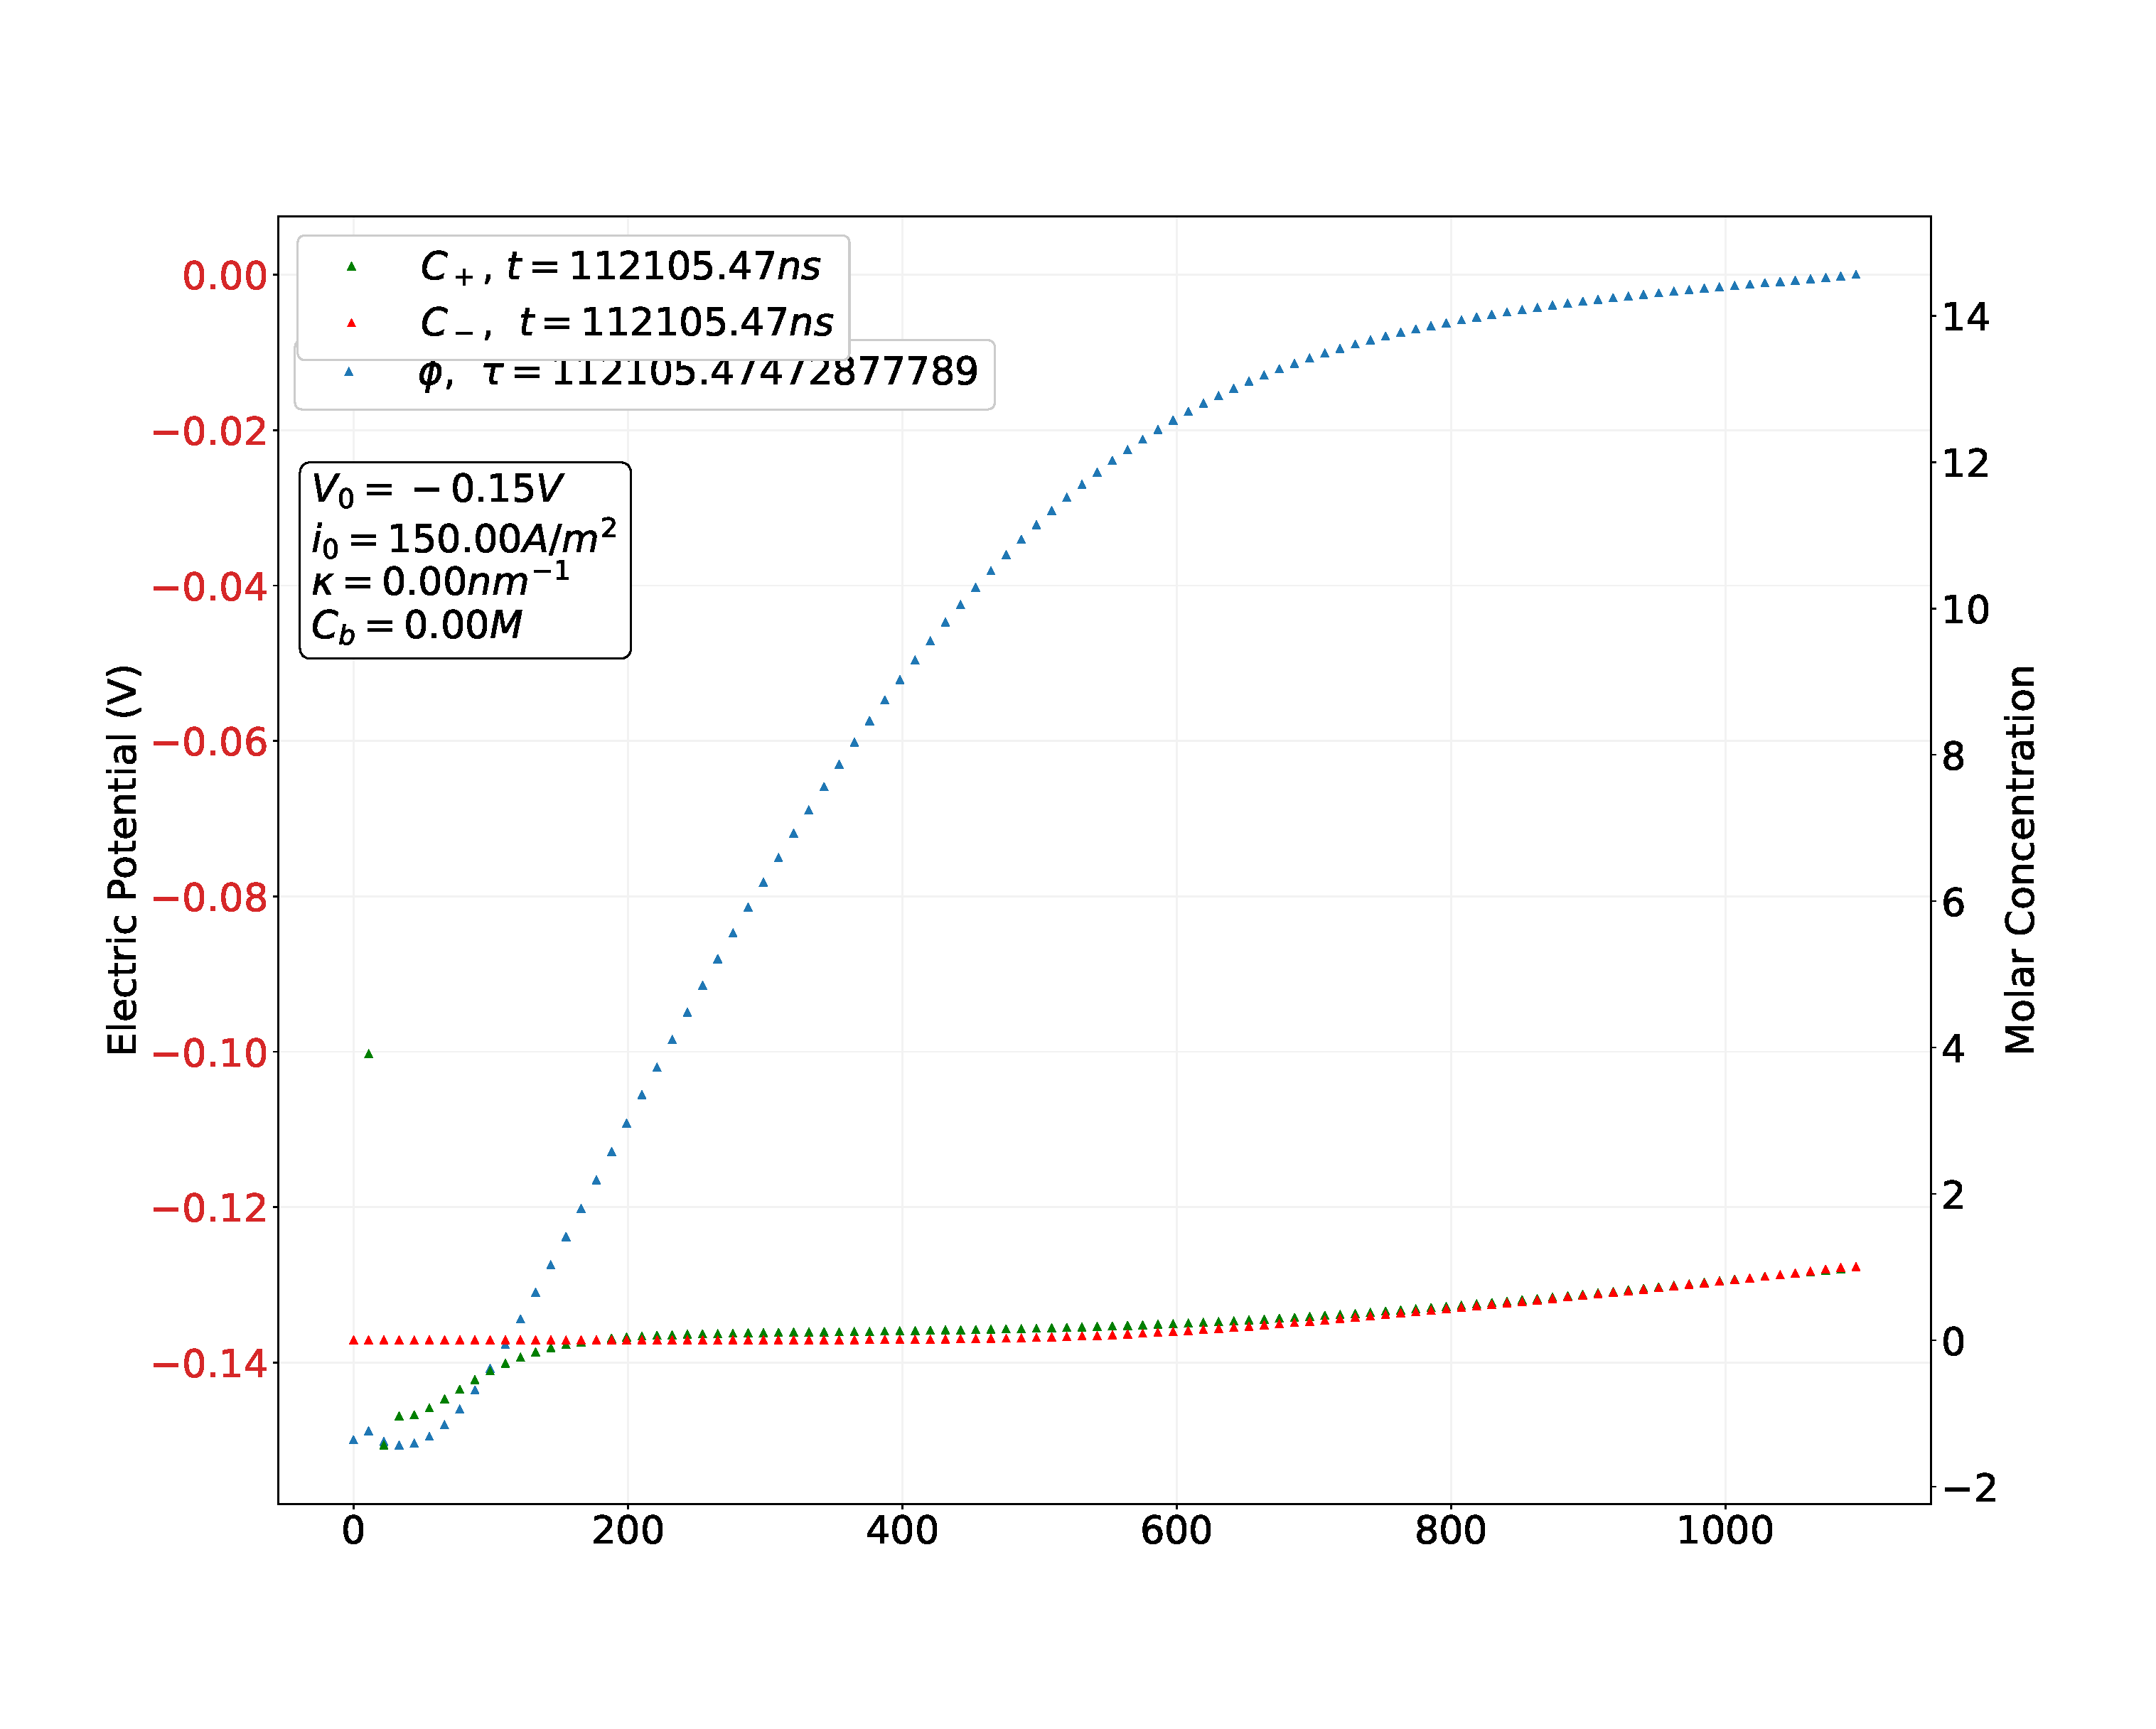
\includegraphics[width =\textwidth]{forced-current-nernstphi1.eps}
\caption{}
\label{fig:ef2}
\end{subfigure}\\[1ex]
\begin{subfigure}{\linewidth}
\centering
\includegraphics[width =0.5\textwidth]{forced-current-nernstphi2.eps}
\caption{}
\label{fig:ef3}
\end{subfigure}
\caption{Electric potential in volts and molar concentration of $Cu^{+2}$ (green dots) and $SO_4^{-2}$ (blue dots) at (a) $t = 0.448 ns$, (b) $t = 2.24 ns$ and (c) $t = 4.44 ns$}
\label{fig:test}
\end{figure}

\newpage

%\subsection{Electric Field At The Surface}

%\newpage
%\subsection{Electric Field Fluctuations At The Surface}



